\chapter{Beam dynamics}

\section{Transversal}


\begin{align}
    \mathbf{\hat{s}}(s) & = \dfrac{d}{ds}\mathbf{\hat{r}}_0 (s), \nonumber \\
     \mathbf{\hat{x}}(s) & = -\rho(s)\dfrac{d}{ds}\mathbf{\hat{s}} (s), \\
      \mathbf{\hat{y}}(s) & = \mathbf{\hat{s}}(s) \times \mathbf{\hat{x}}(s). \nonumber 
\end{align}


\begin{figure}
    \centering
    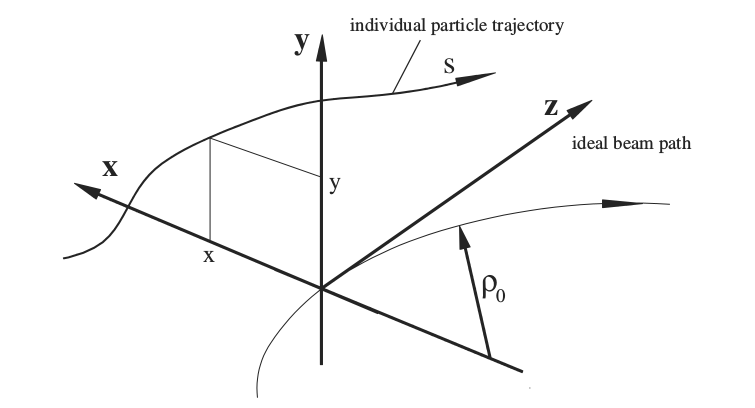
\includegraphics[scale=0.5]{figures/coordinate.png}
    \caption{Curvilinear coordinate system used for storage rings \cite{wiedemann2007physics}}
    \label{sist}
\end{figure}



\begin{align}
    x' & = \dfrac{dx}{ds} \approx  \dfrac{p_x}{p} \nonumber \\
      y' & = \dfrac{dy}{ds} \approx  \dfrac{p_y}{p} \nonumber
\end{align}



\[
z(t) = s_{\text{sinc}}(t) - s(t).
\]



\begin{equation}
    G(s) = \dfrac{1}{\rho(s)} \approx \dfrac{ec}{E_0}B_{y}(s),
\end{equation}



\begin{equation}
    K(s) = \dfrac{e}{p_0} \left.\dfrac{\partial B_y}{\partial x}\right|_{y=0}.
\end{equation}



\begin{align*}
    G(s+C_0) = G(s) \\
    K(s+C_0) = K(s),
\end{align*}



\begin{align*}
    G(s+L) = G(s) \\
    K(s+L) = K(s).
\end{align*}


\begin{equation}
    H_{\perp} = \dfrac{x'^2}{2} + \dfrac{y'^2}{2} + G^2(s)\dfrac{x^2}{2} + K(s)\dfrac{\left(x^2 - y^2\right)}{2} - G(s) x\delta.
\end{equation}



\begin{align*}
   H_x & =  \dfrac{x'^2}{2}  + \left(G^2(s)+K(s)\right)\dfrac{x^2}{2} - G(s) x\delta, \\
   H_y &= \dfrac{y'^2}{2}  -K(s)\dfrac{y^2}{2},
\end{align*}


\begin{align}
    x'' &= - \dfrac{\partial H_{x}}{\partial x}  = -\left(G^2(s) + K(s)\right)x + G(s)\delta, \\
    y'' &= - \dfrac{\partial H_{y}}{\partial y}  = K(s)y.
\end{align}



\begin{align}
    x'' &= -K_x(s)x + G(s)\delta, \\
    y'' &= - K_y(s)y.
\end{align}


\begin{equation}
    x(s) = x_\beta (s) + x_\delta (s),
\end{equation}

\begin{align}
    u'' = -K_u(s) u
    \label{hill}
\end{align}

\begin{align}
    u(s) = \sqrt{2J_u\beta_u(s)}\cos\left(\varphi_u(s) - \phi\right),
\end{align}

\begin{equation}
    \varphi_u'(s) = \dfrac{1}{\beta_u(s)}.
\end{equation}

\begin{equation}
    \nu_u = \dfrac{1}{2\pi} \int_{0}^{C_0} \dfrac{1}{\beta_u(s')}ds'.
\end{equation}

\begin{equation}
    J_u = \gamma_u u^2 + 2\alpha_u u u' + \beta u'^2,
    \label{acao}
\end{equation}

\begin{align}
    \alpha_u(s) &= -\dfrac{1}{2}\beta'(s) \\
    \gamma_u(s) &= \dfrac{1+\alpha^2_u(s)}{\beta_u(s)},
\end{align}

\begin{equation}
    H_\beta = \dfrac{J_x}{\beta_x(s)} + \dfrac{J_y}{\beta_y(s)},
\end{equation}


\begin{align}
    J'_u & = \dfrac{\partial H_\beta}{\partial \varphi} = 0 \Rightarrow J_u = \mathrm{constante}\\
    \varphi'(s) & = \dfrac{\partial H_\beta}{\partial J_u} = \dfrac{1}{\beta(s)}.
\end{align}


\begin{align}
    u(s) &= au(s_0) + bu'(s_0) \\
    u'(s) &= cu(s_0) + du'(s_0)
\end{align}

\[
\left[ \begin{array}{c} 
u(s) \\
u'(s) \end{array} \right] = \left[ \begin{array}{cc} 
a & b \\
c & d \end{array} \right]\left[ \begin{array}{c} 
u(s_0) \\
u'(s_0) \end{array} \right] \rightarrow Y(s) = M(s|s_0)Y(s_0)
\]


\[
\lambda_{\pm} = \dfrac{\mathrm{Tr}\left(M\right)}{2} \pm \sqrt{\left(\dfrac{\mathrm{Tr}(M)}{2}\right)^2 - 1}
\]


\[
\lambda_{\pm} = \cos\mu \pm i \sin\mu = e^{\pm i\mu}.
\]


\begin{equation}
    \mathrm{Tr}\left(M\right) \leq 2
\end{equation}

\begin{equation}
    x_\delta (s) = \eta(s) \delta, 
\end{equation}

\begin{equation}
    \dfrac{\Delta C}{C_0} = \delta\alpha  : = \delta \oint G(s) \eta(s) ds.
\end{equation}

\section{Longitudinal}


\begin{equation}
    \delta U_{\mathrm{rad}} \approx -U_0 - E_0C_0\alpha_z \delta_n
\end{equation}

\begin{equation}
    \omega_{RF} = h\omega_0
\end{equation}

\begin{equation}
    \delta_{n+1} = \delta_n - C_0 \alpha_z \delta_n + \dfrac{V(z_{n+1})-U_0}{E_0}.
\end{equation}

\begin{equation}
    z_{n+1} = z_n + C_0 \alpha \delta_n.
\end{equation}

\begin{align}
    z' & = \alpha\delta(s) \\
    \delta ' & = \alpha_z \delta(s) + \dfrac{V(z(s))-U_0}{C_0E_0}.
\end{align}

\begin{equation}
    H_{||} = \dfrac{\alpha}{2}\delta^2 + \Phi(z),
\end{equation}

\begin{equation}
    \Phi(z) := -\dfrac{1}{C_0 E_0}\int_0^z \left(V(z') - U_0\right)dz',
\end{equation}

\begin{equation}
    \dfrac{\partial \Psi}{\partial s} + \left\{\Psi , H\right\}  = \mathcal{F}\left(\Psi\right)
\end{equation}

\[
H = H_\beta + H_{||} =  \dfrac{J_x}{\beta_x(s)} + \dfrac{J_y}{\beta_y(s)} + \dfrac{\alpha}{2}\delta^2 + \Phi(z),
\]


\begin{align}
    f_x(J_x) & = \dfrac{1}{2\pi \epsilon_x}\exp\left(-J_x/\epsilon_x\right) \\
    f_y(J_y) & = \dfrac{1}{2\pi \epsilon_y}\exp\left(-J_x/\epsilon_y\right) \\
    f_{\delta}(\delta) & = \dfrac{1}{\sigma_{\delta}\sqrt{2\pi}}\exp\left(-\delta^2/2\sigma^2_\delta\right) \\
    \lambda(z) & = \lambda_0\exp\left(-\Phi(z)/\sigma^2_\delta\alpha\right)
    \label{dist}
\end{align}

\begin{align}
    \epsilon_x & = \dfrac{D_x c}{2 \alpha_x} \\
    \epsilon_y & = \dfrac{D_y c}{2 \alpha_y} \\
    \sigma_\delta & = \dfrac{D_z c}{2 \alpha_z} 
\end{align}


\begin{align}
    \sigma_x^2(s) & = \langle y^2 \rangle = \int y^2 f_{y}(y) dy = \beta_y(s) \epsilon_y\\
    \sigma_x^2(s) &= \langle \left(x_\beta + \eta \delta \right)^2 \rangle = \beta_x(s) \epsilon_x + \eta^2 \sigma_\delta^2.
\end{align}

\chapter{LOCO}

LOCO é uma sigla em inglês para Linear Optics from Closed Orbits, um algoritmo proposto por J. Safranek em 1997 \cite{safranek}. Este método utiliza distorções da órbita fechada dos elétrons dada perturbações dipolares localizadas para extrair informações sobre a ótica linear. 

A perturbação dipolar é aplicada por ímãs dipolares dedicados chamados de corretoras, cuja principal função é corrigir as distorções de órbita. Existem corretoras horizontais (CH) e verticais (CV). A órbita é medida também nos planos horizontal $x$ e vertical $y$ em pontos longitudinais do anel, utilizando dispositivos chamados Beam Position Monitors (BPMs). No anel de armazenamento do Sirius há 120 CHs, 160 CVs e 160 BPMs.

É possível medir a resposta da órbita em $x$ e $y$, dada uma variação da força de uma corretora individualmente. A força de uma corretora é chamada de kick, denotada pelor $\theta$ e dada em ângulo. Se normalizarmos a distorção de órbita $\Delta r$ medida em cada BPM pela variação de kick aplicado, para cada corretora, podemos construir uma matriz independente do kick aplicado, chamada de matriz resposta de órbita.

\begin{equation}
    M_{ij} = \dfrac{\Delta r_i}{\Delta \theta_j}.
\end{equation}

Esta matriz resposta de órbita possui $2 \times n_{\mathrm{BPM}}$ linhas (medidas horizontais e verticais) e $n_\mathrm{{CH}} + n_{\mathrm{CV}}$ colunas. Para anel de armazenamento do Sirius, a matriz resposta tem dimensão $(320 \times 280)$. 

No Sirius, tipicamente a variação de kick dipolar usada na medida é da ordem de dezenas de $\mu$rad e a correspondente variação de órbita é da ordem de dezenas de $\mu$m. A maior contribuição da matriz vêm dos termos bloco-diagonais, isto é, distorção horizontal (vertical) de órbita dada uma variação de corretora horizontal (vertical). Os termos não-diagonais são distorções horizontal (vertical) de órbita dada uma variação de kick dipolar vertical (horizontal) e estão relacionados ao acoplamento transversal entre os dois planos. Idealmente no regime de acoplamento transversal nulo, os termos não-diagonais são nulos.

É possível calcular uma expressão analítica para os elementos da matriz resposta \cite{wiedemann2007particle}:

\begin{align}
M_{ij} &= \dfrac{\sqrt{\beta(s_i)\beta(s_j)}}{2\sin\pi\nu}\cos\left[ |\varphi(s_i) - \varphi(s_j)| - \pi\nu \right],
\label{matriz}
\end{align}

onde $\beta(s)$ é a função bétatron (beta) em uma coordenada longitudinal $s$, $\varphi(s)$ o avanço de fase bétatron e $\nu$ a sintonia bétatron do anel. Os parâmetros são horizontais $x$ ou verticais $y$ de acordo com o plano do elemento da matriz. Na eq. \eqref{matriz} observa-se que a matriz resposta depende das funções beta e do avanço de fase ao longo do anel, portanto depende da chamada ótica linear. 

Para implementar o algoritmo LOCO é necessário ter um modelo computacional do acelerador, em que é possível calcular numericamente a matriz resposta. Variações nas forças dos quadrupolos da rede magnética (portanto nas focalizações), alteram a ótica do anel, logo também alteram a matriz resposta. A ideia principal do algoritmo LOCO é calibrar parâmetros relevantes do modelo simulado de forma a minimizar a diferença entre a matriz resposta calculada numericamente e a matriz resposta medida no anel real. Após esta calibração, induz-se que a ótica linear do modelo simulado representa a ótica linear do anel real, portanto os resultados de correções de ótica simuladas neste modelo calibrado podem ser traduzidos e aplicados na máquina real, com o objetivo de corrigir a ótica na prática. 

Um ponto muito importante de se mencionar é que este algoritmo depende muito que a modelagem computacional do acelerador seja o mais fiel possível ao acelerador real, sobretudo em relação ao posicionamento dos elementos magnéticos e de diagnóstico.

O objetivo do método é minimizar iterativamente a quantidade:

\begin{equation}
    \chi^2 = \sum_{ij} \left(M^{\mathrm{medida}}_{ij} - M^{\mathrm{modelo}}_{ij}\right)^2 = \sum_{{k = (i,j)}} V_{k}^2,
\end{equation}

onde $V_{k}$ é a diferença vetorizada das matrizes, tendo $2 \times n_{\mathrm{BPM}} \times (n_\mathrm{{CH}} + n_\mathrm{{CV}})$ elementos organizados em forma de vetor. Para o anel do Sirius este vetor tem $2 \times 160 \times 280 = 89600$ entradas. Se $\vec{V}$ é dependente de parâmetros $\vec{P}$, podemos expandir em primeira ordem:

\begin{equation}
V_{k}(\vec{P}^{n+1}) = V_{k}(\vec{P}^{n}) + \sum_{l}\dfrac{\partial V_{k}}{\partial P_{l}} \Delta P_{l}^{n},
\label{taylor}
\end{equation}

onde $n$ denota a iteração do algoritmo. Podemos escrever a eq. \eqref{taylor} matricialmente como:

\begin{equation}
    \Delta \vec{V}  = J_{\mathrm{LOCO}} \Delta \vec{P},
\end{equation}

onde $J_{LOCO}$ é a matriz jacobiana cujos elementos são $J_{kl} = \dfrac{\partial V_{k}}{\partial P_{l}}$.

O algoritmo LOCO busca resolver o problema iterativamente com $\vec{V}^{n+1} + \Delta \vec{V}^n = 0$. Com isto, podemos calcular a variação dos parâmetros que minimizam o vetor $\vec{V}$ por:

\begin{equation}
    \Delta \vec{P}^{n+1} = J_{\mathrm{LOCO}}^{-1} \vec{V}^{n}.
\end{equation}

e aplicá-los nos parâmetros da máquina. 

Genericamente a matriz $J_{\mathrm{LOCO}}$ é retangular (o número de linhas igual ao número de elementos da matriz resposta de órbita e o número de colunas igual ao número de parâmetros a serem ajustados). Desta forma o símbolo $J_{\mathrm{LOCO}}^{-1}$ representa uma pseudo-inversa, obtida através de decomposição em valores singulares (SVD). Este jacobiano é calculado numericamente e pode tomar boa parte do tempo de execução do algoritmo dependendo das dimensões do problema.

Em resumo, o objetivo do LOCO é encontrar o mínimo global de uma função de $p$ variáveis, onde $p$ é o número de parâmetros a serem ajustados (dimensão do vetor $\vec{P}$), dadas $k$ equações, onde $k$ é o número de elementos da matriz resposta de órbita. Para aceleradores modernos $p$ é um número da ordem de $10^{2} \sim 10^{3}$ e $k$ da ordem de $10^4$. Isto caracteriza o LOCO como um problema superdeterminado, onde o número de equações supera o número de incógnitas por uma ou mais ordens de grandeza.